\begin{figure}[h!]
  \center
  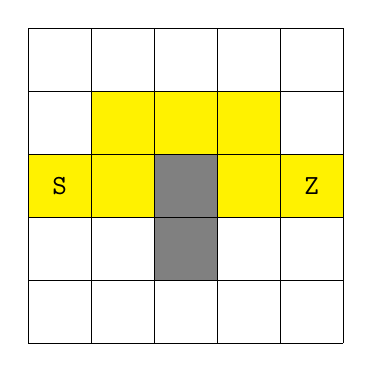
\begin{tikzpicture}
    [
      scale=0.8,
      every node/.style={black},
      path/.style={fill=yellow},
      wall/.style={fill=gray},
    ]

    \draw[step=1cm] (0,0) grid (5,5);

    \draw [wall] (2,2) rectangle (3,3);
    \draw [wall] (2,1) rectangle (3,2);
    
    \draw [path] (0,2) rectangle (1,3) node [midway, font=\ttfamily] {S};
    \draw [path] (1,2) rectangle (2,3);
    \draw [path] (1,3) rectangle (2,4);
    \draw [path] (2,3) rectangle (3,4);
    \draw [path] (3,3) rectangle (4,4);
    \draw [path] (3,2) rectangle (4,3);
    \draw [path] (4,2) rectangle (5,3) node [midway, font=\ttfamily] {Z};
  \end{tikzpicture}
  \caption{Wegfinde-Algorithmus}
  \label{fig-pathfinding-example}
\end{figure}